% !TEX root = SystemTemplate.tex

\chapter{Overview and concept of operations}

This document will look at the Lounge Against the Machine team's third sprint for building
a program tester. Looking at the team members and their roles, the project
management that we used, the sprint retrospective, any terminology or acronyms
that we use. Next we will look at the user stories, backlog and requirements of the
program. Then we will look at the design and implementation of the program focusing
on major pieces of the code. The next section will look at system and unit testing of 
our program, followed by development environment, and release, setup and
deployment of our program. We will finish this document with a look at a user 
documentation (including a user guide, installation guide and programmer manual)
class index and class documnetation.


\section{Scope}
This document will cover the third sprint of our program tester built for Dr. Logar's
software engineering class in Spring 2014 .


\section{Purpose}
The purpose of this program is to compile, run and test the simple programs created by others. The program willl also offer to generate additonal random tests.

\subsection{Normal Run}
The programs it tests are guaranteed to compile and run correctly. It will then search through a root directory, find each student's
subdirectory, compile their code into the root directory, open log files for the student and the class as a whole. Student logs will
go into the student's directory and the class log will be in the root. The student logs will have the results of each test, a final
score, and results from running GNU tools gprof and gcov on the program. The final score will be based on the precent of the tests passed. A program may be marked as a fail if it fails a critical test, or times out. Critical tests are labeled as "crit\_(something).tst".

\subsection{ Generate Tests}
The program will ask for a number tests to generate, the number of inputs for
each test, and the data type for the tests. The program will then generate a "GeneratedTests" directory in the test directory of the root
folder. At which point, the program will generate the number of tests specified. If the program has previously generated tests, it will
then remove the past generated tests and create new ones. 


\section{Systems Goals}
1) Find student programs to compile.\\
2) Find the tests and use them to test the found programs.\\
3) Generate new random test cases.\\
4) Log information about the test runs, including pass percentage, code coverage, and code performance.

\section{System Overview and Diagram}
The program will be started on the command line. You may specify a testing directory. If a testing directory is not supplied, the program will assume its current directory is the testing directory. It will then display a simple menu for executing existing test cases, generated new test cases, or exiting.  See Figure~\ref{systemdiagram}.

\begin{figure}[tbh]
\begin{center}
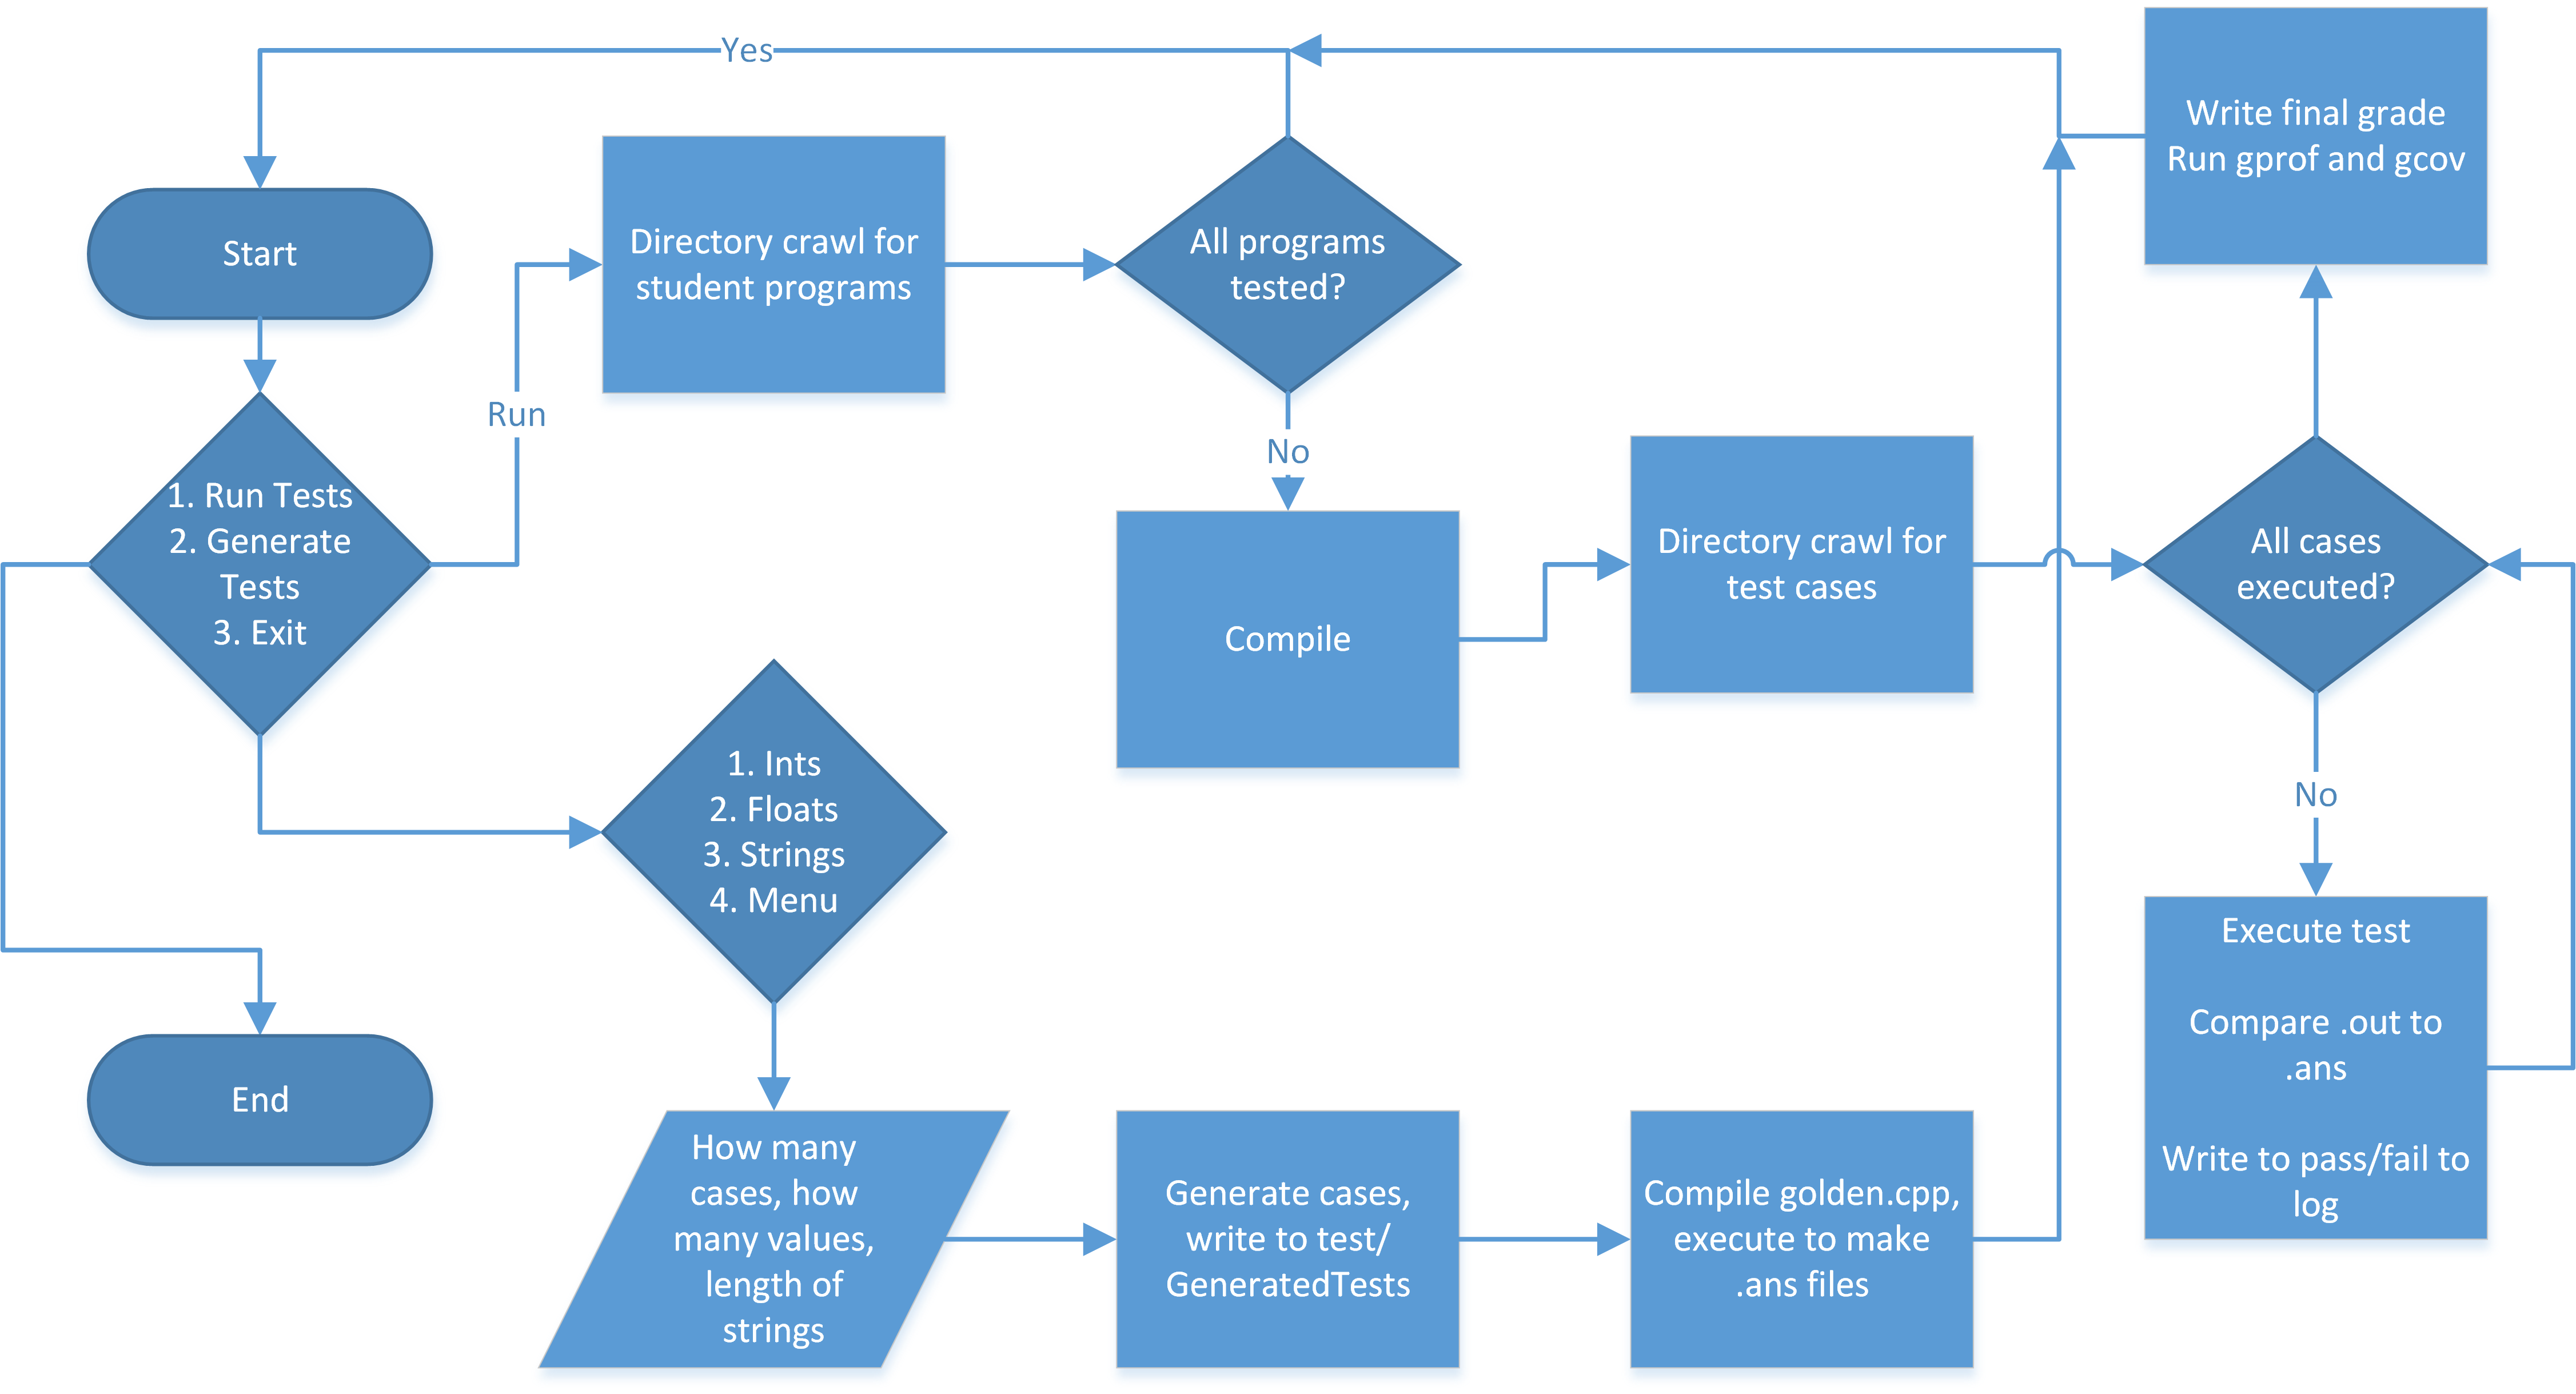
\includegraphics[width=0.75\textwidth]{./SystemDiagram}
\end{center}
\caption{System Diagram \label{systemdiagram}}
\end{figure}

\section{Technologies Overview}
The program was written in C++, and was compiled with g++ on a linux environment. The program also requires use of GNU tools gprof and gcov. Project management was done through Trello. Source control was done through GitHub. Documentation was created using \LaTeX.
